Our Alloy analysis focuses on the production data release and analysis and what they involve. The main goals of the model are the following : 
\begin{itemize}[label=\textbullet]
	\item Define correct rules for (in)complete productions releases and (not) confirmed batches, so that the list of farmers with "confirmed"status is up-to-date.
	\item Define rules to get this list of farmers full at the end of the croping season.
	\item Define rules to provide help to every farmer who performed badly during the previous season.
\end{itemize}

\lstinputlisting[language=alloy]{dream.als}


\begin{figure} [!h]
	\centering
	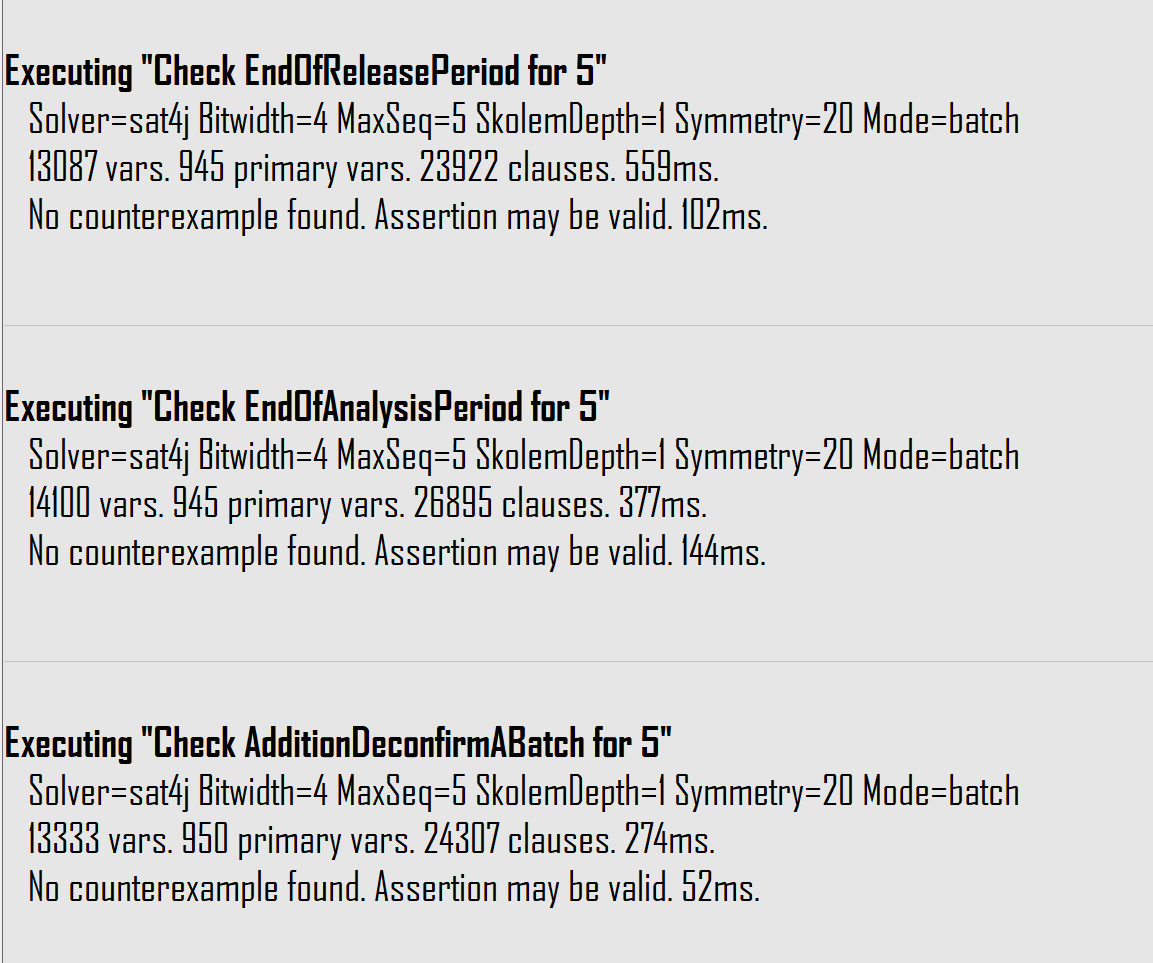
\includegraphics[width=0.5\textwidth]{Images/alloy-check-results.png}
	\caption{\label{fig:seq} Results of the check commands}
\end{figure}

\begin{figure} [!h]
	\centering
	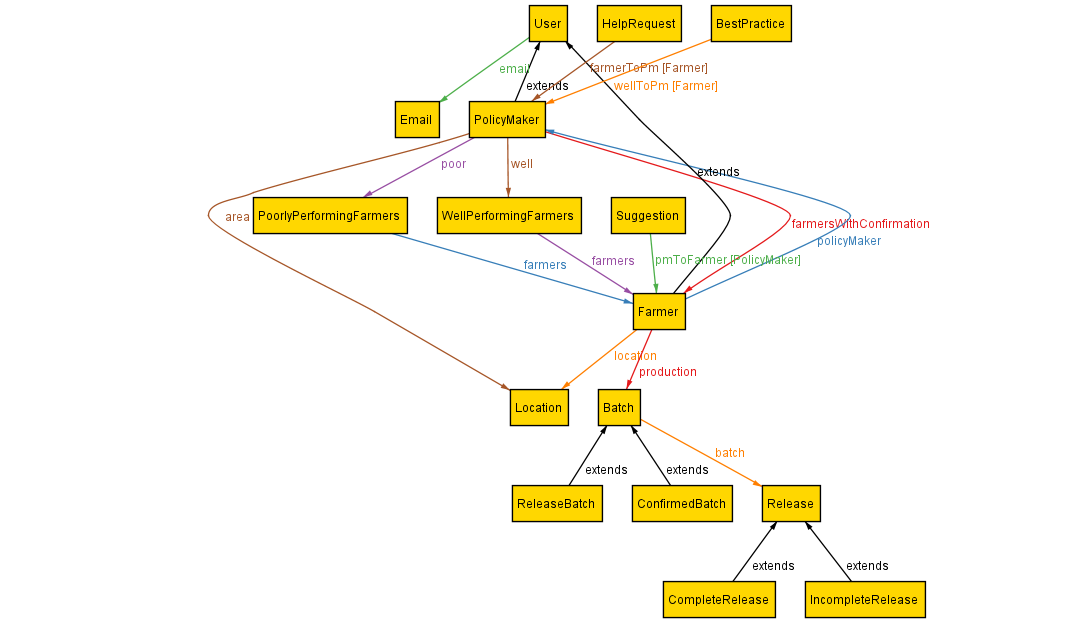
\includegraphics[width=1.2\textwidth]{Images/alloy-metamodel.png}
	\caption{\label{fig:seq} Meta Model}
\end{figure}